\section{Results: evidence by requirement}
\label{sec:evidence}

Each subsection gives the answer for one requirement, the tally of codes and the studies behind it.
The code, comparator and rationale of every study--requirement pair are in the released coding data (\oa{B}).
``\jev{}'' means the hosted model (\texttt{jev-1.13} where a study reports a version). Open models are named.
\Cref{fig:framework} summarises the codes and \cref{tab:keyfindings} the key findings with their certainty.

\begin{figure}[t]
\centering
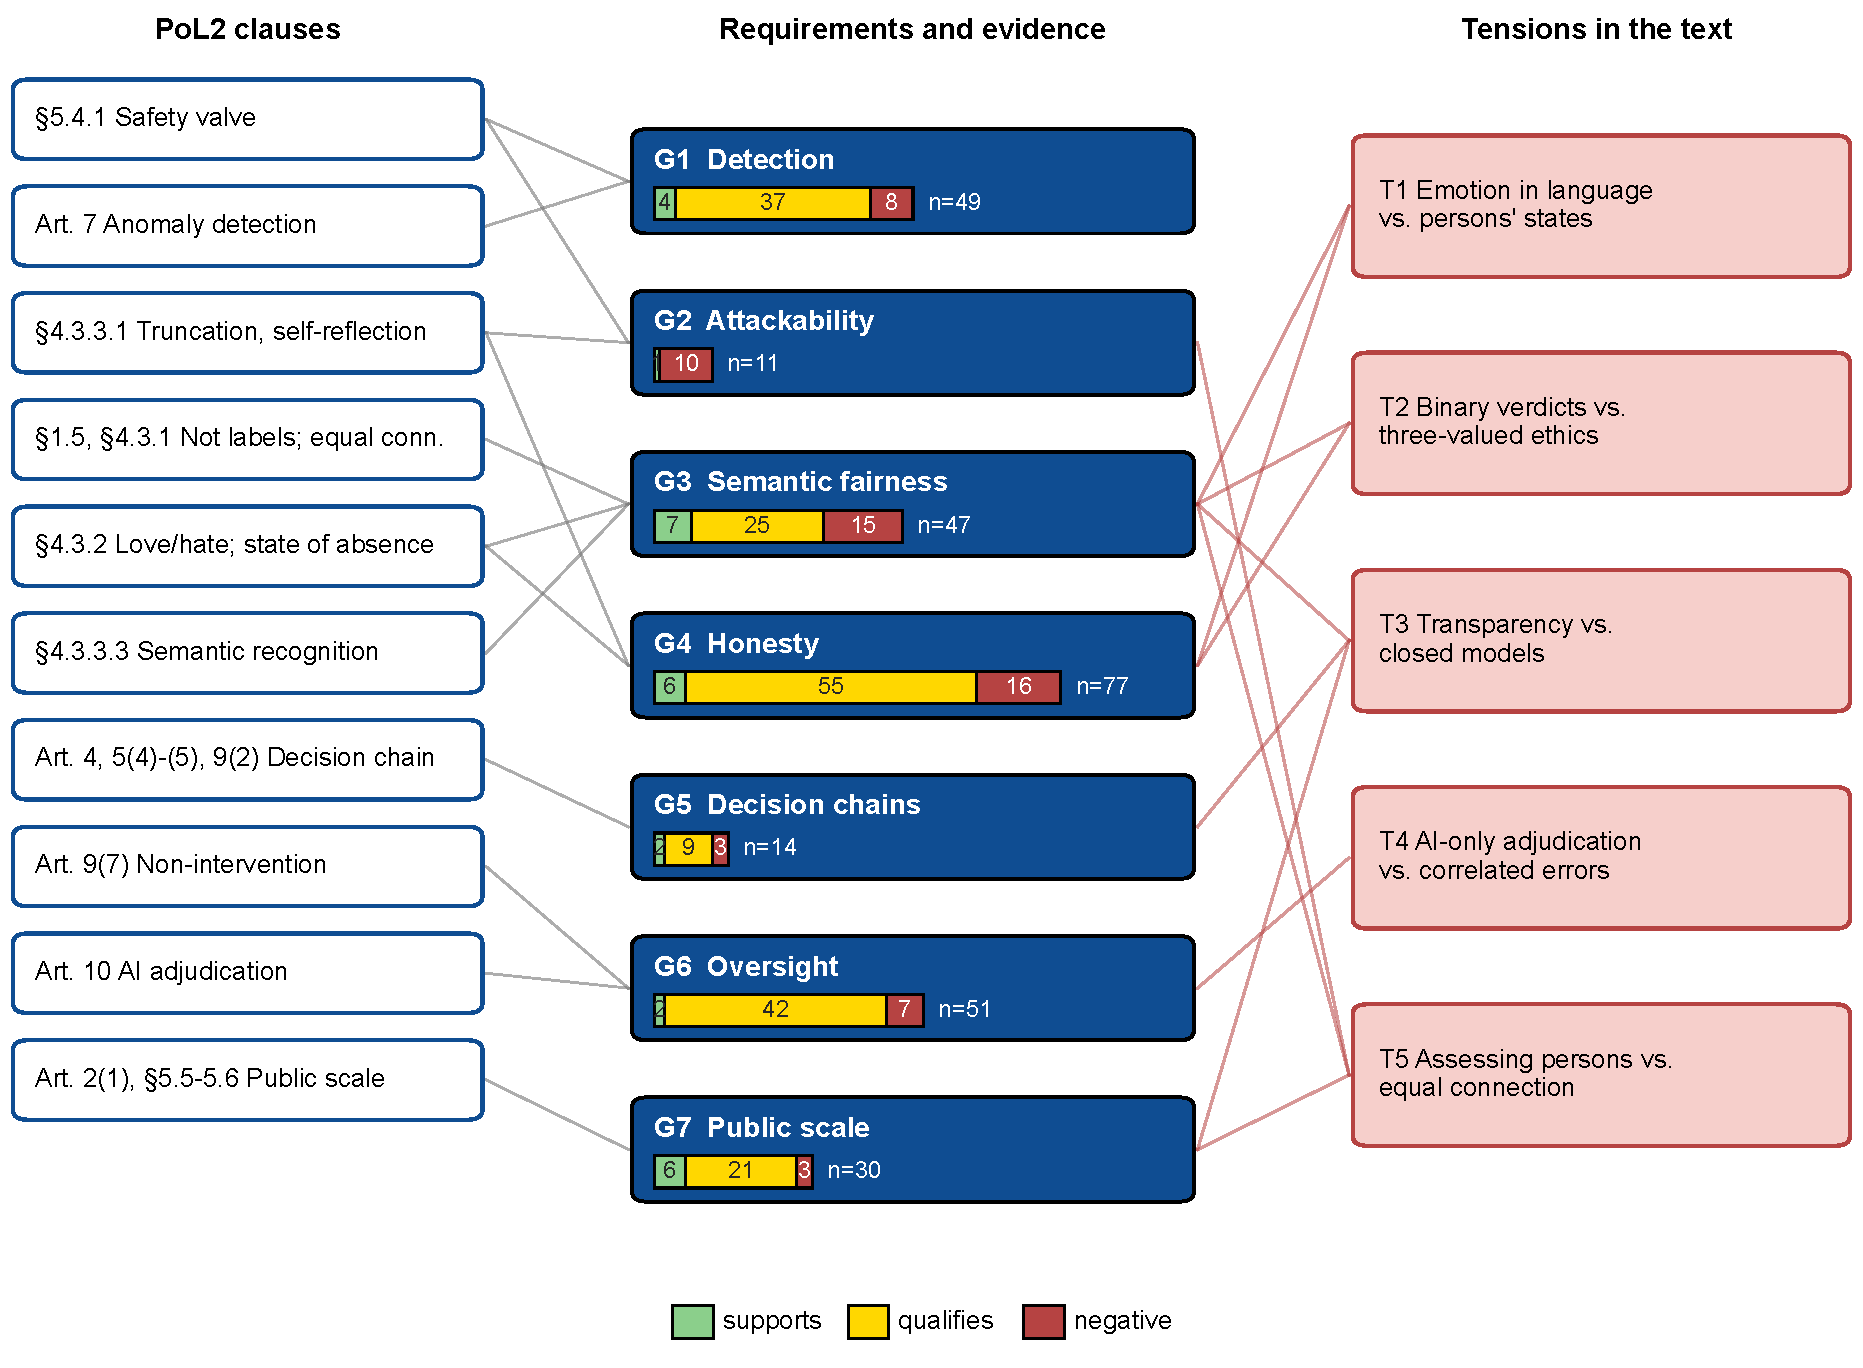
\includegraphics[width=0.95\linewidth]{figures/fig_framework.pdf}
\caption{From clauses to tensions. Left: \pol{} clauses that require or constrain machine judgement. Middle: the seven requirements and the codes of the studies informing each, for detector use (supports, qualifies, negative; \oa{B}); bars count studies and do not measure effect size or certainty, and non-empirical items are excluded. Right: the five tensions of \cref{sec:synthesis}, linked to the requirements whose evidence they cite.}
\label{fig:framework}
\end{figure}

\subsection{G1 --- Detection}
\label{sec:g1}

\emph{Yes as a ranking, not yet as a decision} (S~4, Q~37, N~8).
On English benchmarks typed models rank harmful or misaligned content well, at a small fraction of the cost of generative evaluators.
Without training, a single generic yes/no question to \jev{} reached a median AUROC of 0.886 (95\% CI 0.821--0.952) over 31 alignment-failure benchmarks, and on the 19 benchmarks scored by an API LLM evaluator it cost \$0.30 against \$18.96 per pass~\cite{arx29429}.
\jev{} had the highest AUROC of the low-cost generative evaluators on six binary tasks~\cite{zen22885291}\zmark{}, but was often below the best ones. It trailed the best LLM on 14 of 15 preregistered annotation tasks, by a median of 11.6 macro-F1 points~\cite{arx24574}.
On hate speech, without task training, commercial LLMs were significantly ahead of every decision model on only one of four English datasets, but every system separated hate from merely offensive language weakly (three-class macro-F1: \jev{} 0.532, a frontier LLM 0.604, a supervised TF-IDF classifier 0.639)~\cite{arx03324}.
Selecting which hate-speech policy a post violated was harder: \jev{} chose the exact policy in 29.4\% of cases without retrieved precedents (51.6\% with them)~\cite{arx07953}.
In a single-run study that classifies the emotion expressed in texts, not persons' states, every system was weak on Chinese emotion classification (macro-F1: \jev{} 21.06, generative models 19.82--23.31)~\cite{arx08829}.
Thresholds fitted in one setting fail in another. Median F1 rose from 0.706 at the default threshold to 0.822 at a cross-validated one, mostly on benchmarks with rule- or evaluator-scored labels; on human-validated labels the default did as well (0.721 against 0.694)~\cite{arx29429}.
A reproduction of five of its benchmarks found the extreme case on TensorTrust hijacking, with AUROC 0.95 but F1 0.158 at the default threshold of 0.5 and 0.947 at a threshold fitted by cross-validation~\cite{jkf87_2026replication}\gmark{} (\cref{fig:fragility}a).
Errors concentrate in sub-types that aggregate scores hide. In agent-security screening \jev{} missed all 130 prompt injections that carried no explicit instruction, and made 130 of its 167 misses on that benchmark at confidence $\geq 0.95$~\cite{arx33401}.
In an agent harness it screened injections well (AUROC 0.98) yet passed 25.5\% of harmful requests~\cite{arx02267}.
On numeric signals the evidence is weaker still: zero-shot \jev{} scored below always predicting the majority class on network-flow features~\cite{arx00376}, and in industrial fault detection under shift it did no better than flagging every window~\cite{arx09937}.
Against generative comparators the typed models were better or similar in 11 of 36 pairs, mixed in 17 and worse in 8.
These results match what was known for probability-reading safety classifiers~\cite{inan2023llama,rottger2021hatecheck}, except that ranking every message is now cheap enough to run on all traffic.

\begin{figure}[t]
\centering
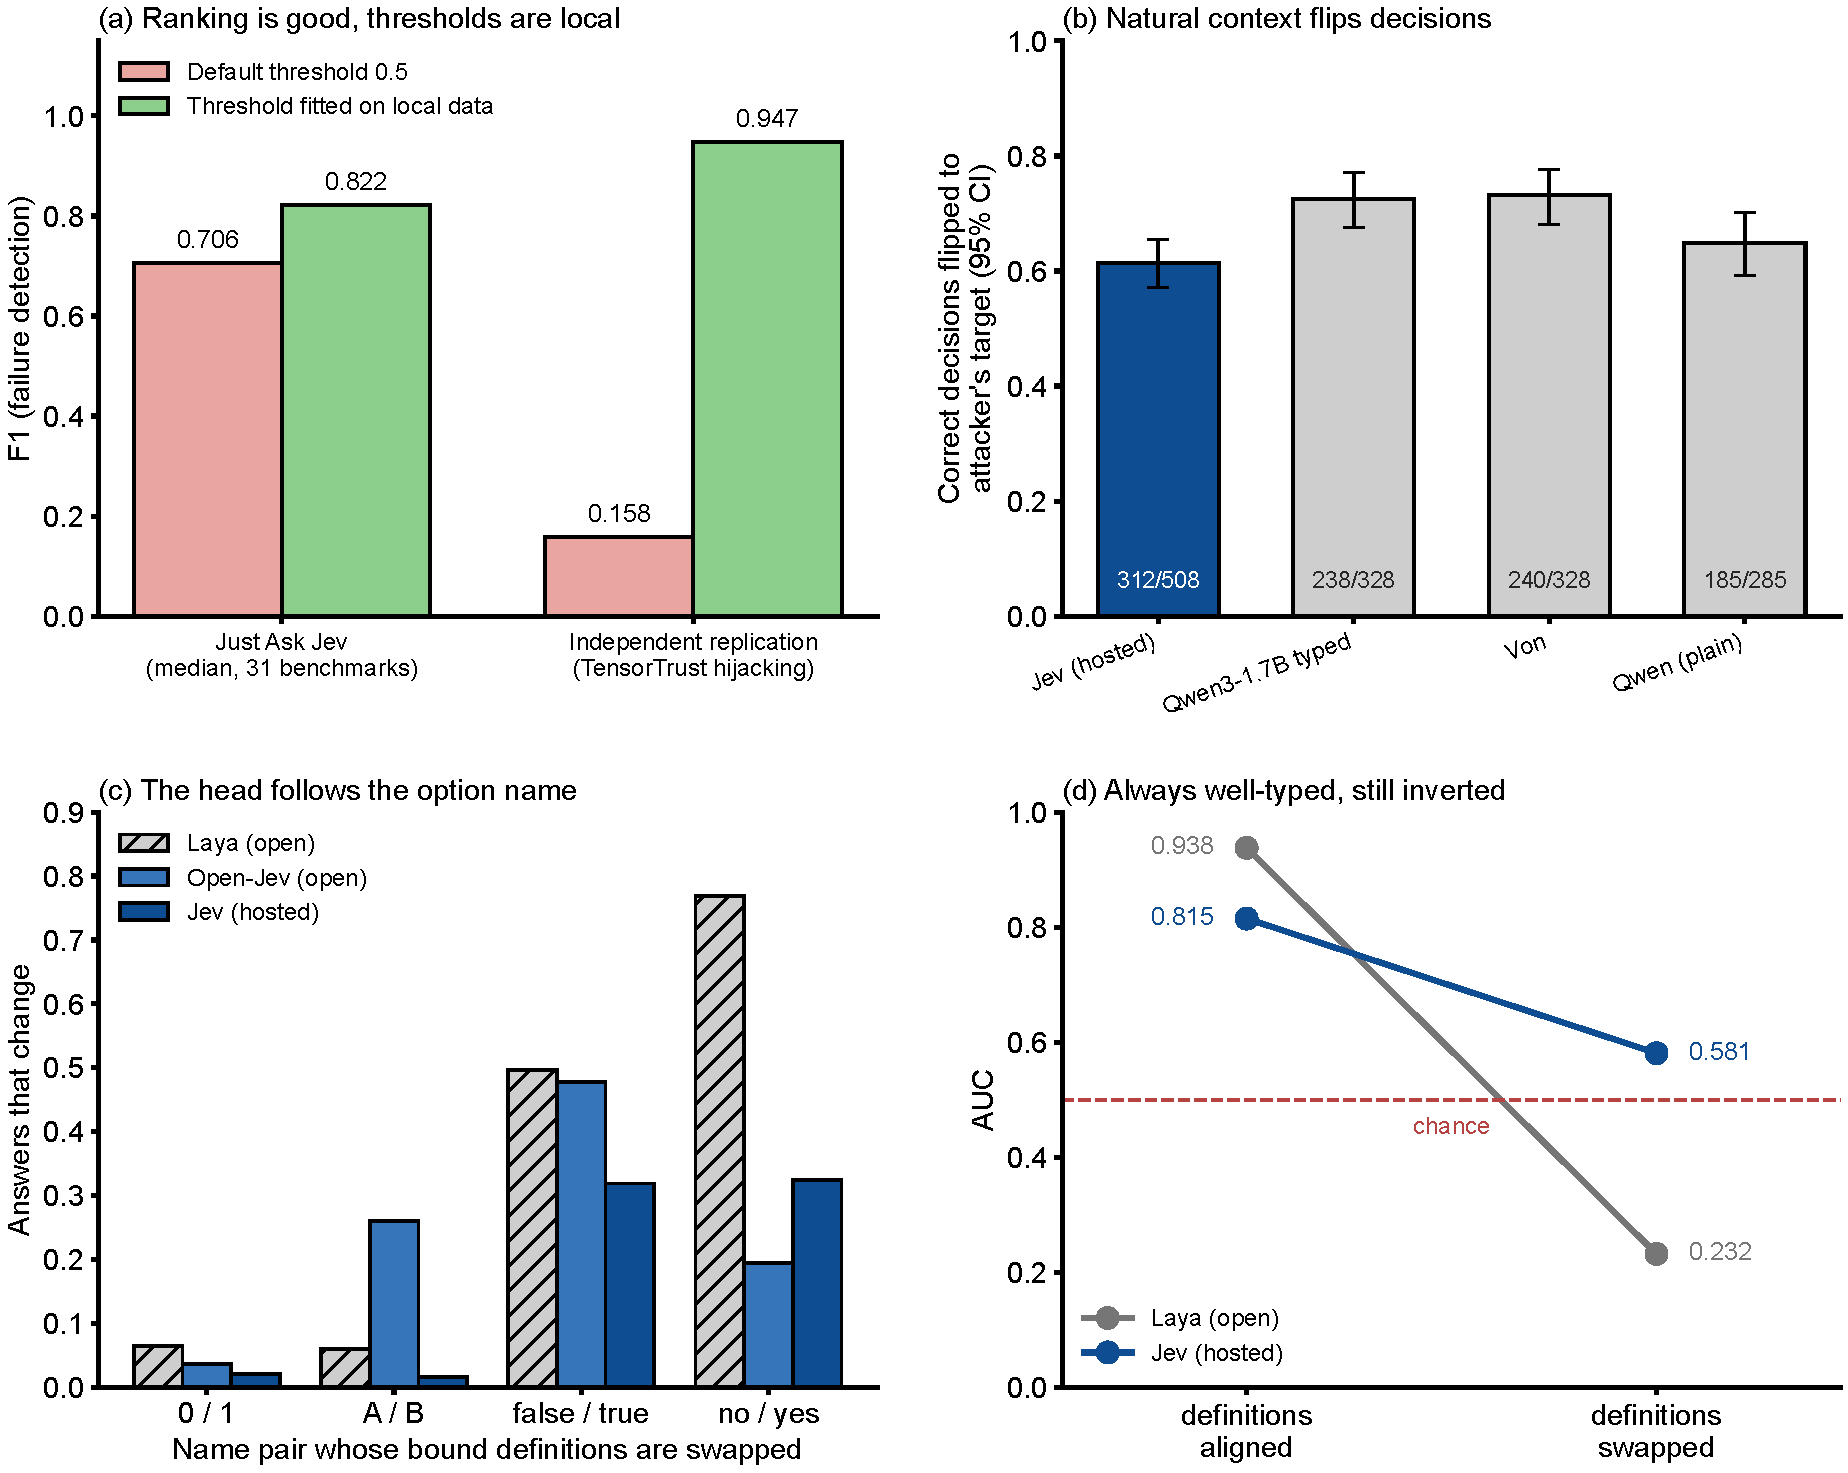
\includegraphics[width=0.9\linewidth]{figures/fig_fragility.pdf}
\caption{G1--G3: a detector, and a fragile one.
(a) F1 at the default threshold versus a threshold fitted on local data~\protect\cite{arx29429,jkf87_2026replication}.
(b) Share of initially correct decisions redirected to an attacker-chosen wrong option by optimised fluent context additions, each system on its own correct items; ``Von'' is an open typed model evaluated in that study; error bars are Wilson 95\% intervals from the reported counts~\protect\cite{arx30243}.
(c) Share of answers that change when the definitions bound to a pair of option names are swapped, with question, state, names and definition texts unchanged; Open-Jev over 1{,}800 questions, Laya and \jev{} over 1{,}200~\protect\cite{arx26758}.
(d) AUROC with the \texttt{yes/no} definitions aligned with or swapped between the names; the type-error rate is 0\% throughout~\protect\cite{arx26758}.
Panels (a) and (b) use \texttt{jev-1.13.0} or the \texttt{jev-latest} alias; the study in (c)--(d) does not report the hosted version.}
\label{fig:fragility}
\end{figure}

\subsection{G2 --- Attackability}
\label{sec:g2}

\emph{Yes, the content under review can steer the safeguard} (S~1, Q~0, N~10; the most consistently negative requirement).
Every study that attacked a typed model with the content it was asked to judge had some success, and several successful attacks used content that looked ordinary.
One unverified observer opinion appended to the state flipped 12.1\% of \jev{}'s decisions (CI 8.5--15.5), statistically tied with impersonating an authority~\cite{arx31142}.
Short fluent context additions, searched with the model's own probabilities, redirected 61.4\% of initially correct \jev{} decisions to an attacker-chosen wrong option, while three other decision systems were redirected on 64.9--73.2\% of theirs~\cite{arx30243} (\cref{fig:fragility}b).
A \jev{}-specific injection and a universal suffix reached 97--100\% attack success on three tasks~\cite{arx04985}.
Where the correct action required an unstated inference, words in the state that echo an option acted as lures~\cite{arx01834}.
The strongest of three adaptive multi-turn agents succeeded in 25 of 27 runs against one \jev{}-based application (version not reported), in what its authors call a directional study of one application~\cite{checkpoint2026jev}\gmark{}.
The one supporting study found that injected instructions selected the attacker's target in only 1.8\% of cases (3.5\% for an adaptive attacker)~\cite{arx28613}, but the other attacks on \jev{}, which used different attacks and benchmarks, contest this finding.
Other systems attacked in the same studies were also vulnerable. One study shows a weakness specific to typed models: the probability vector that makes them useful also guides the attacker (63.6\% success against 56.4\% with labels only)~\cite{arx30243}.

\subsection{G3 --- Semantic stability and fairness}
\label{sec:g3}

\emph{Not by default} (S~7, Q~25, N~15).
Decisions can follow the names of options rather than the definitions bound to them.
Swapping only which definition is bound to \texttt{yes} and \texttt{no}, with question, state, option names and definition texts fixed, changed 32.5\% of the answers of hosted \jev{} (version not reported), about 24 times its test--retest floor. The same swap inverted the AUROC of the open Laya model from 0.938 to 0.232, an inversion that a type check cannot detect~\cite{arx26758} (\cref{fig:fragility}c--d).
Under a matched harness the same swap flipped 50.5 of every 100 answers of \jev{}, while digit or random-string identifiers brought it near its noise floor~\cite{arx00346}.
Decisions also depend on option order and wording~\cite{arx38827,zen23023694}\zmark{}, and without a persona \jev{} answered a cross-cultural values survey like its own American personas~\cite{arx36399}.
Robustness varies by model. Hosted \jev{} was less affected than Laya but more than some larger open decoders~\cite{arx00346}.
In Chinese, a repository benchmark found that hosted \jev{} changed 1.9\% of voice-routing and 2.9\% of customer-service decisions under option-order swaps and 1.7\% between simplified and traditional script ($n = 323$; the open Laya model 10.8--20.6\% under order swaps)~\cite{qin2026zhdecisionbench}\gmark{}.
On a second Chinese benchmark, however, built by the authors of Laya-based Chinese models, hosted \jev{} (version not reported) had a calibration error of 11.45\% on general tasks against 3.78\% for the authors' model, though in specialised domains \jev{} was the better calibrated (5.57\% against 12.08\%)~\cite{arx36965}.
The vendor states that CJK languages are handled ``but not equally well''~\cite{typesafe_models}. No study tests \pol{}'s constructs.

\subsection{G4 --- Honesty}
\label{sec:g4}

\emph{Partly} (S~6, Q~55, N~16).
Hosted \jev{} is often well calibrated on familiar closed-choice tasks (pooled ECE 0.028 for Choice questions over 37 datasets~\cite{arx37647}), usually better than generative models' stated confidence and mixed against frontier models~\cite{arx24574,arx34024}.
However, calibration is local. Recalibration on local labels reduced ECE substantially~\cite{arx24052,arx27607}, and on the items where annotators disagreed most, the ECE of its Choice probabilities rose to 0.339, against 0.076 on the most agreed quarter, although in that preregistered study it was far better calibrated than a local generative baseline~\cite{zen23032384}\zmark{}.
Related probabilities need not cohere. For ``the label is X'' and ``the label is not X'' the two probabilities deviated from summing to one by 0.064 on average, five times \jev{}'s repeat noise~\cite{arx33209}.
The answer ``insufficient'' is rarely reported when it should be. Offered ``I don't know or cannot answer'' on a medical benchmark, \jev{} chose it on 10.5\% of the items for which it was the correct answer, and ``None of the above'' on 53.9\% of the items where that was correct (a frontier generative model: 8.6\% and 73.9\%)~\cite{arx34024}.
When recognising that every listed answer was wrong required arithmetic, it chose ``None'' on only 7\% of items~\cite{arx39496}.
In one study, a separate yes/no question asking whether the evidence suffices detected missing information on multi-hop questions better than confidence (AUROC 0.95 against 0.85). As a filter for accepting answers, however, it was 2--6 points less accurate than confidence~\cite{arx01006}.
Against generative comparators the typed models were better in 15 of 34 pairs and worse in 5.

\subsection{G5 --- Decision chains}
\label{sec:g5}

\emph{Recorded and decomposed, not explained} (S~2, Q~9, N~3).
A typed decision returns a probability and nothing else, so nothing in its output shows which part of the input produced a verdict~\cite{willison2026jev}.
Decisions assembled from several questions or interfaces need not cohere. Asked through two interfaces, the same decision led to different actions in 32.8\% of cases (a post-trained open model: 34.2\%)~\cite{arx37470}.
Writing intermediate facts into the state makes chains inspectable and, when those facts are right, can make them more accurate.
When \jev{}'s prediction of an opponent's move was written into the state, its decisions in misleading games rose from 33\% to 94\% correct. Given a wrong written premise, however, it followed the premise in 24 of 26 calls, so the written facts themselves become the audit points~\cite{arx01834}.
Decomposition does not always help. Splitting a judgement into criterion questions combined by a fixed rule did not raise accuracy in two studies~\cite{arx03324,arx08829}, while exposing only the fields relevant to each step, or moving checks into a separate gate, raised correct decisions in two others~\cite{arx07327,arx06425}.

\subsection{G6 --- Oversight and escalation}
\label{sec:g6}

\emph{It depends on where escalation goes and how thresholds are set} (S~2, Q~42, N~7).
Escalating uncertain cases to a stronger reasoning model, or accepting only verdicts that an independently built rule confirms, saved a quarter to over half of the cost without loss of accuracy in several studies~\cite{arx26550,arx24574,arx02048}.
One study contests the escalation result: a \jev{} pre-screen cut an LLM safety reviewer's cost by only 4.3\% once its own tokens were counted~\cite{arx02267}.
Escalating to peer models preserved confident errors. On \jev{}'s 12 most confident errors on each of seven grading panels, three low-cost generative evaluators gave \jev{}'s wrong answer in 242 of 252 verdicts (96.0\%, against 50.3\% expected if errors were independent). Because these items were selected as confident errors, this is an upper bound on error correlation, though it is the set that matters for escalation~\cite{arx29769}.
Thresholds fixed in advance missed their error targets on new data in most studies that set one. In a preregistered annotation study, a confidence threshold of 0.9 that was to give at least 0.85 accuracy fell short on 8 of 14 tasks~\cite{arx24574}.
In several studies, however, \jev{}'s threshold met its target, among them a preregistered study of changed question types in which its gate, set in advance, stayed within its target on 6 of 7 templates~\cite{arx33689}.
Unlike most earlier work on cascades~\cite{chen2023frugalgpt,goel2025great}, these studies separate the two cases: a differently constructed rule helped as the second check, and a peer model did not.

\subsection{G7 --- Public scale}
\label{sec:g7}

\emph{Cheap, and possible to do honestly, under conditions} (S~6, Q~21, N~3).
Typed models make population-scale reading and simulation cheap, and some studies show how to do it honestly.
One simulator called \jev{} once per unique state and propagated the measured human--model discrepancy as a shared error term into every conclusion. This gave retrospective coverage of 0.93 and 0.96 at nominal 80\% and 90\% on 37 unseen studies, although its preregistered primary endpoint showed no clear gain~\cite{arx27535}.
A statewide study read about half a million police narratives and audited a probability-stratified sample by blind human adjudication~\cite{arx00213}.
However, simulated publics lean towards one population and understate disagreement~\cite{arx36399,zen23032384}\zmark{}, residual personal identifiers survived two redaction passes~\cite{arx00213}, and deployment depends on one closed vendor that does not offer the model for self-hosting~\cite{arx28919}.
Typed safeguards can also leak what they read. Conditional instructions planted in user input made hosted \jev{}'s labels alone reveal hidden gender, age-group, heart-disease and ethnicity attributes in every tested case, and 200 of its labels trained a surrogate model to 92\% agreement~\cite{arx04985}.

\subsection{Across requirements}
\label{sec:across}

Of the \nRowsAll{} coded study--requirement pairs, \nSAll{} support detector use, \nQAll{} qualify it and \nNAll{} are negative. The shares change by four points or less when only stronger-design studies are kept or Zenodo records are dropped.
\nComparedAll{} pairs compared a typed model with a generative evaluator on the same requirement. The typed model did better in \nCompBetter{}, similarly in \nCompSimilar{}, mixed in \nCompMixed{} and worse in \nCompWorse{}.
For failures the evidence is thinner and less favourable. Of the \nNegComp{} negative codes with a comparator, the typed model was worse in \nNegCompWorse{}, similar in \nNegCompSimilar{}, mixed in \nNegCompMixed{} and better in \nNegCompBetter{}, and \nNegNoComp{} of the \nNegAll{} negative codes had no comparator at all.
The evidence therefore does not show that typed models are generally worse than generative evaluators, nor that their failures are shared with them.
Almost every success depended on an added condition, such as a locally fitted threshold, a second independent check or human review, and the failures in G2 and G4 are failures of the detector itself.
The argument of \cref{sec:design} is therefore that the failures of typed detectors are cheaper to contain in a detector role, where every consequential action passes another check, than in a judge role, where none does.

\begin{table}[!htbp]
\centering
\footnotesize
\setlength{\tabcolsep}{3pt}
\caption{Key findings and the certainty of the evidence. \emph{Scope}: hosted \jev{}, open models, or both (typed models generally); findings about hosted \jev{} or both are rated on hosted-model evidence alone, counted per system arm. \emph{Codes}: the supporting studies' codes. \emph{Sources}: the principal supporting, then opposing studies; ``open:'' open-model studies, which corroborate (or, ``against'', point the other way) but do not enter the rating. Certainty under the rules of \cref{sec:method}; $^{c}$~contested within the scope; $^{j}$~descriptive tally rated by judgement. Every study counted for each finding, with its direction and design, is listed in \oa{C}; the ratings are computed by \nolinkurl{scripts/rate_certainty.py}.}
\label{tab:keyfindings}
\begin{tabularx}{\linewidth}{@{}L>{\raggedright\arraybackslash}p{0.06\linewidth}>{\raggedright\arraybackslash}p{0.055\linewidth}>{\raggedright\arraybackslash}p{0.13\linewidth}>{\raggedright\arraybackslash}p{0.22\linewidth}>{\raggedright\arraybackslash}p{0.08\linewidth}@{}}
\toprule
Finding & Scope & Codes & vs.\ generative & Sources & Certainty \\
\midrule
Ranks harmful or misaligned content well zero-shot at a fraction of the cost; often less accurate than the best LLMs & hosted & S/Q/N & better (low-cost); worse (best) & \cite{arx29429,jkf87_2026replication,zen22885291,arx33401,arx24574,arx27678} & low \\
Fixed thresholds do not transfer; local fitting is needed & both & Q & -- & \cite{arx29429,jkf87_2026replication,arx00346,arx01006,arx26550,arx24574,arx02046,arx03387,arx02267,zen22935043}; opposing: \cite{arx33689} & low$^{c}$ \\
Errors concentrate in sub-types hidden by aggregates & hosted & Q & mixed & \cite{arx33401,alphaRAG,arx02046,arx07953,arx03324,arx08675,arx10321} & low \\
Inserted opinions, optimised context and lexical lures steer decisions & both & N & similar & \cite{arx31142,arx01834,arx01006,arx30243,arx02048}; open: \cite{zen22959854,zen23038928} & low \\
Instruction injection rarely selects the attacker's target (1.8\% raw, 3.5\% adaptive) & hosted & S & -- & \cite{arx28613}; opposing: \cite{arx31142,checkpoint2026jev,arx04985} & very low$^{c}$ \\
Option names can override definitions; neutral identifiers remove most of it & both & N & -- & \cite{arx26758,arx00346,arx07953}; open: \cite{arx02586} & low \\
Defaults to one culture's values & hosted & N & -- & \cite{arx36399} & very low \\
Well calibrated on familiar closed-choice tasks, mixed against frontier models; calibration is local & hosted & S/Q & better or mixed & \cite{arx37647,arx01006,arx24052,arx27607,arx24574,arx34024,zen22885291} & low \\
Explicit ``I don't know'' rarely chosen when correct; ``none'' inconsistently & hosted & Q/N & similar or worse (frontier); worse (reasoning) & \cite{arx34024,arx39496,arx01006,arx03387,arx06425} & low \\
A separate sufficiency question detects missing information, but filters answers less well than confidence & hosted & Q & -- & \cite{arx01006} & very low \\
Escalation to a stronger reasoner saves cost without loss of accuracy on readable judgements & both & Q & similar & \cite{arx26550,arx24574,arx02046}; opposing: \cite{arx02267}; open: \cite{zen22922769}; open, against: \cite{arx07177,arx03324} & low$^{c}$ \\
Acceptance on agreement with an independently built rule lost no macro-F1, but fewer disguised attacks were flagged & both & Q/N & similar & \cite{arx02048}; open: \cite{zen22904595} & very low \\
Peer evaluators repeat \jev{}'s most confident errors (upper bound) & hosted & N & similar or mixed & \cite{arx29769,arx33401} & low \\
Thresholds set in advance miss error targets on new data & both & Q/N & -- & \cite{arx33401,arx24574,arx03387,arx02267}; opposing: \cite{arx33689,zen22935043,zen23075657}; open: \cite{arx33843,zen23041163,arx07177} & low$^{c}$ \\
Typed models are not generally worse than generative evaluators; most failures lack a comparison & both & -- & \nCompBetter{} better, \nCompWorse{} worse of \nComparedAll{} & coding data (\oa{B}) & low$^{j}$ \\
No study measures the \pol{} construct (three-valued, Chinese) & -- & -- & -- & -- & -- \\
\bottomrule
\end{tabularx}
\end{table}
